\chapter{ Аналитический раздел}
\label{cha:analysis}

\textit{SDR(Standart Dynamic Range) изображение}\cite{bib1} -- изображение, пиксели которого содержат цвета и яркость, максимальная глубина которых 8 бит.

\textit{LDR(Low Dynamic Range) изображение}\cite{bib1} -- изображение, пиксели которого хранят ограниченный диапазон цветов и яркости, предназначенное для отображении на мониторах с глубиной цвета 8 бит или меньше.

\textit{HDR(High Dynamic Range) изображение}\cite{bib2} -- изображение, пиксели которого содержат более широкие значения цвета и яркости в сравнении с изображениями стандартного диапазона(SDR), глубина цвета которых больше 8-ми бит.

\textit{Глубина цвета} -- количество бит, приходящихся на один пиксель 

\section{ Различия LDR и HDR изображений}
    
    Несмотря на то, что технологии за последние несколько лет быстро развиваются и качество полученных кадров и устройств, их отображающих, увеличивается, получение картинки, сопоставимой с реальным окружением, остается нелегкой задачей. Яркость, диапазон цветов, которые видит человек в повседневной жизни, невозможно отобразить на большинстве мониторов.

    Хотя уже начинают появлятся так называемые HDR мониторы и существуют камеры, сенсоры которых позволяют запечатлить широкий спектр цветов, яркостей и деталей, цена таких устройств очень большая, поэтому большинство мониторов остаются SDR формата и не в состоянии передать картинку с большим количеством цветовой информации.

    Глубина цвета на большинстве мониторов составляет 8 бит. Глубина цвета самого распространенного формата изображений JPEG так же составляет 8 бит, в котором используется цветовое пространстов $YC_rC_b$\cite{bib1}. Это цветовое пространство позволяет использовать лишь малую часть видимых человеком цветов. Так же это цветовое пространство не способно передать большую часть яркостей, которых способен распознать человеческий глаз.

    В противовес формату JPEG существует так называемый RAW формат. В отличии от JPEG он способен содержать гораздо больше информации. Глубина цвета такого формата может достигать 12-16 бит(Значение может варьироваться в зависимости от возможностей сенсора камеры), который доступен в большинстве современных камер. Чаще всего этот формат автоматически переводят в JPEG во время съемки, что приводит к потере многих деталей без возможности восстановления. Однако, используя специальные инструменты RAW изображение в дальнейшем можно преобразовать в LDR изображение, получив на выходе кадр без потери нужной информации(провести tonemapping)\cite{bib1}.

    На цветовом пространстве \ref{fig:hdrdiff} наглядно показан охват возможных отображаемых цветов в RGB пространстве или на тех же LDR мониторах и в HDR с глубиной цвета хотя бы в 12 бит.

\begin{figure}[ht!]
    \centering{
        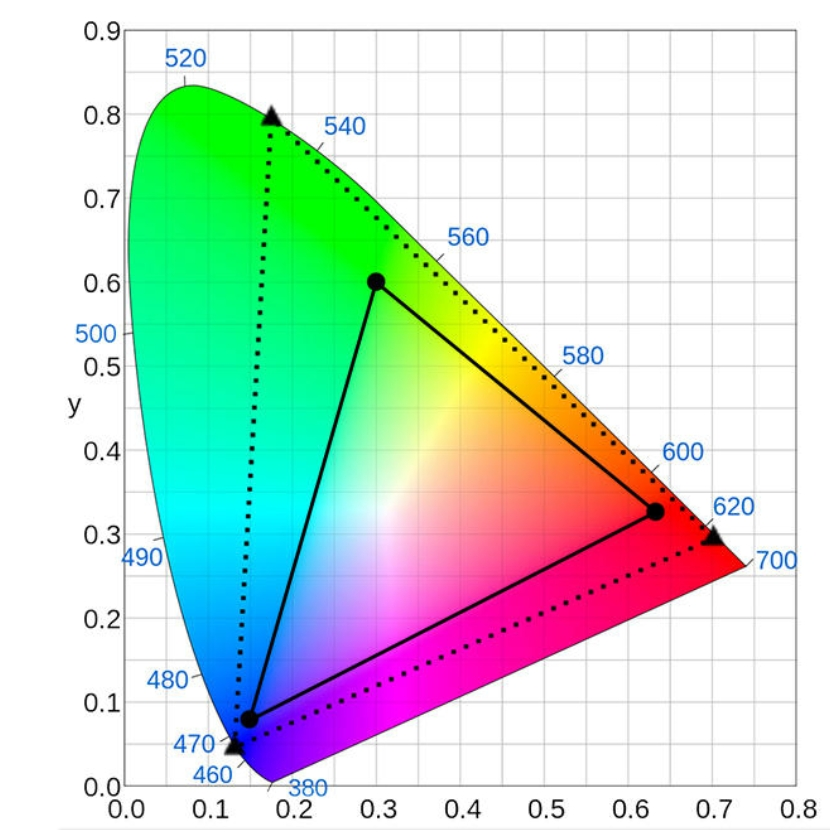
\includegraphics[width=0.4\textwidth]{img/rgb_vs_hdr_gamut.jpg}
	\caption{Охват видимых человеком цветов цветовым пространством RGB и HDR.}
        \label{fig:hdrdiff}
        }
\end{figure}

    Главное различие HDR и традиционных LDR изображений\cite{bib1} в том, что HDR картинка не зависит от какого-либо устройства и содержит максимально большое количество информации. Количество отображаемой информации на устройстве уже зависит непосредственно от его собственных характеристик и возможностей. LDR изображение же зависит от устройства, на котором оно будет отображаться и спроектировано специально под мониторы или экраны, которые отображают определенное количество цветовой информации.

\section{ Процесс получения HDR изображения}

HDR изображение можно получить несколькими способами\cite{bib1}: 
\begin{itemize}
    \item c помощью объединения снимков с разной длинной экспозиции,
    \item с помощью камеры, сенсор который позволяет захватить широкий объем данных,
    \item при помощи перевода LDR изображения в HDR специальными алгоритмами
\end{itemize}

Первый метод является более распространенным, так как устройства, которые больше всего распространены в повседневной жизни(телефоны, планшеты, веб-камеры) не обладают достаточно мощными сенсорами, для того, чтобы захватить широкий диапазон цветов. Последний метод не получил распространения, потому что задача перевода LDR или SDR изображения в HDR возможна только при помощи преминения алгоритмов реконструкции, завязанных на нейронных сетях, появившихся достаточно недавно.

\subsection { Метод получения HDR изображения на камере со слабым сенсором}
\begin{itemize}
    \item Выравнивание кадров,
    \item Реконструкция и удаление движущихся объектов(артефактов),
    \item Слияние кадров с разной экспозицией,
    \item Преобразование HDR к LDR(tonemapping) если это требуется
\end{itemize}

Наглядно процесс получения HDR кадра с возможностью перевода его в LDR\cite{bib3} показан на рисунке \ref{fig:hdrpipeline}

\begin{figure}[ht!]
    \centering{
        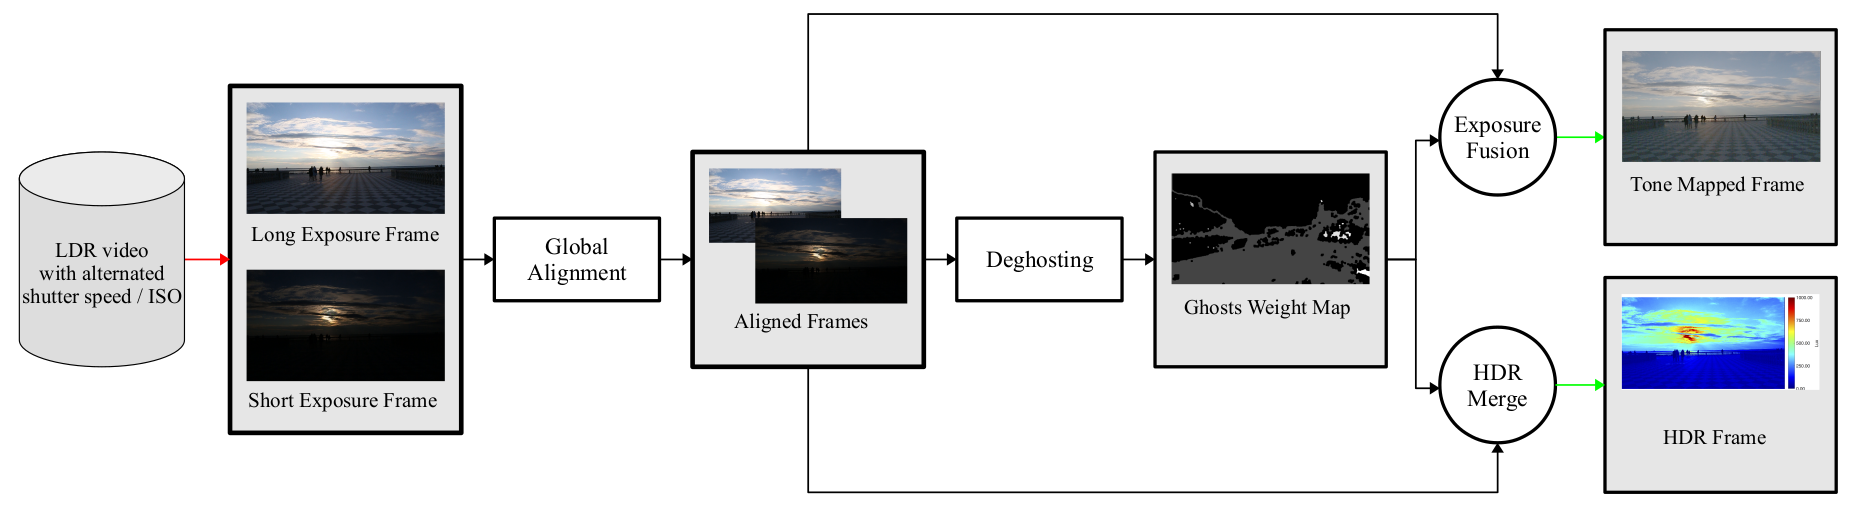
\includegraphics[width=1\textwidth]{img/hdrpipeline.png}
	\caption{Процесс получения HDR изображения путем слияния кадров с разной экспозицией}
        \label{fig:hdrpipeline}
        }
\end{figure}

\subsection{ Получение HDR видео на камере со слабым сенсором в режиме реального времени}
    
    Данная задача подразумевает собой быстрое создание HDR изображений из 2-3 кадров с изменяещейся экспозицией, которые получаются, путем изменения экспозиции через каждый последующий кадр. Таким образом, можно быстро получить два кадра, которые будут содержать всю информацию о самых темных и самых светлых участках сцены. Так, как эти кадры следуют друг за другом, различия в них, предполагается, будут незначительными.

    При записи видео в таком формате очень важна скорость алгоритмов, использующихся при получении HDR кадра. Операции выравнивания, удаления артефактов, слияния кадров и преобразование полученного кадра в LDR должны протекать быстро.

\subsubsection{ Способы получения разной экспозиции в видео}
    Получение разной экспозиции кадров можно добиться несколькими способами\cite{bib1}:
\begin{enumerate}
    \item Использовать несколько камер, каждая из которых будет вести запись с соответствующей экспозицией;
    \item Использовать камеру с нескольким сенсорами, каждыдй из которых будет вести запись с соответствующей экспозицией;
    \item Использовать одну камера, меняя параметр выдержки или ISO, которые влияют на полученную экспозицию;
\end{enumerate}

    Первые два способа позволяют сохранить количество кадров в секунду и улучшить качество получаемой картинки, но они требуют предварительной калибровки. Так же несколько камер и камеры с дополнительными сенсорами не самые распространенные решения в телефонах и других гаджетах.
    
    Третий способ позволяет получать кадры с разной экспозицией на любом устройстве, в котором есть камера, что делает его более универсальным, но это снижает количество кадров в секунду почти в два раза.

\section{ Выравнивание изображений}
    Первым шагом в получении HDR изображения является глобальное выравнивание последовательности кадров с разной экспозицией. Предполагается, что 2 соседних кадра не меняются слишком быстро.

    Но при съемке с рук или при съемке в движении, кадры все равно меняются, положение записывающего устройства тоже может быть нестабильным. В дальнейших шагах получения HDR снимка очень важно, чтобы кадры с разной экспозицией были максимально выровнены по отношению друг к другу. 

    Задача выравнивания усложняется тем, что экспозиции изображений сильно разнятся. Для решения этой задачи используется алгоритм MTB(Median Threshold Bitmap)\cite{bib4} пороговое отсечение по медианному значению.

\subsection{ Алгоритм MTB(Median Threshold Bitmap)}
    На вход алгоритму подается N 8-битных монохромных изображений, которые можно получить путем использования зеленого канала изображения, либо путем перевода каждого пикселя 24-битного sRGB изображения в серый цвет с помощью выражения \ref{eq:grayscale}
\begin{equation}
    \centering{
        grey = \frac{(54*red + 183*green + 19*blue)}{256}}
    \label{eq:grayscale}
\end{equation}

    Одно из изображений выбирается базовым. Остальные N-1 при выравнивании будут опираться на базовое.

    Далее требуется для каждого из изображений:
\begin{enumerate}
    \item Найти медианное значение(8-битное значение) из гистограммы низкого разрешения пикселей монохромного изображения. 
    \item Создать растровое изображения, в котором 0 будут отмечаться пиксели, которые меньше или равны медианному значению и 1 будут отмечаться пиксели, которые строго больше этого медианного значения.
\end{enumerate}

    Результаты этоих шагов представленны на примере двух изображений с разной экспозицией \ref{fig:bitmapExample}

\begin{figure}[ht!]
    \centering{
        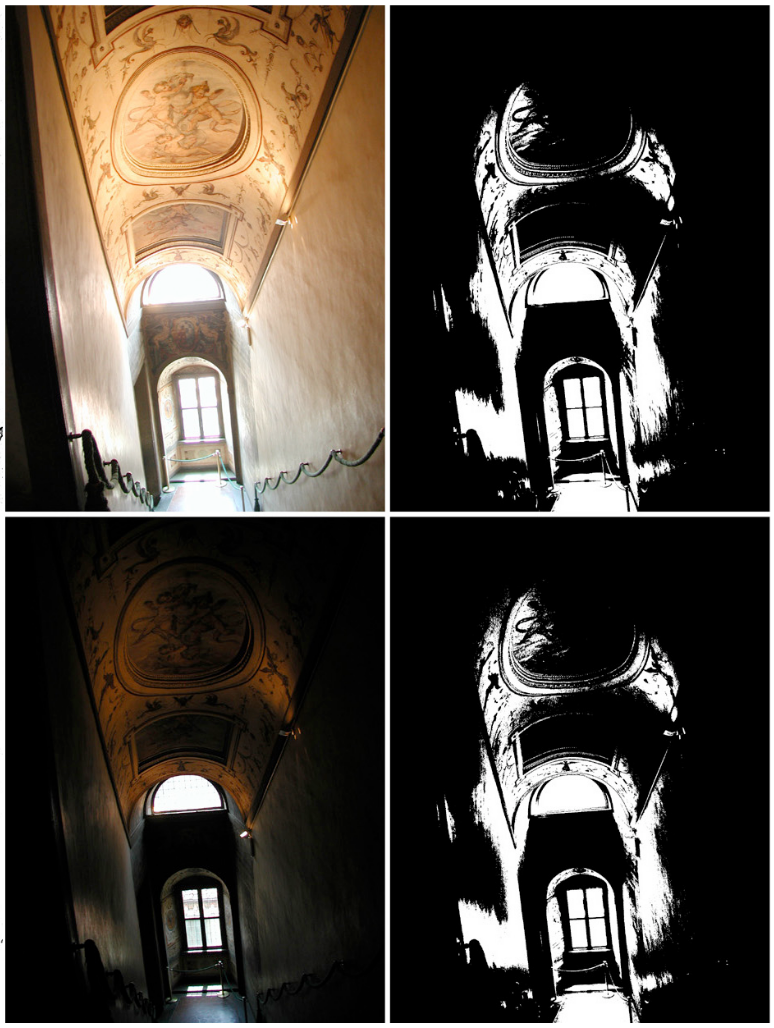
\includegraphics[width=1\textwidth]{img/bitmapExample.png}
	\caption{ Получение растровых изображений, использующихся для дальнейшего сравнения(справа), оригиналы изображений(слева)}
        \label{fig:bitmapExample}
        }
\end{figure}

    После этого каждое N-1 изображение подгоняется под базовое. Вначале они сравниваются. Сравнение происходит путем побитовой операции XOR -- каждый пиксель изображения высчитывается с каждым соответствующем пикселем базового изображения операцией XOR. Результаты сохраняются и на выходе получается очередное растровое изображение, в котором 0 - пиксели, информация которых совпала с базовым изображением и 1 - пиксели, информация которых не совпала.

Для устранения шумов, которые могут получиться при съемке в темных, плохо освещенных помещениях, используется \textit{исключающее растровое изображение}. Т.к. шумы возникают близко к медианному значению, пиксели, лежащие на расстояние ближе чем 4 пикселя к медианному значению не учитываются. 

Так генерируется исключающее растровое изображение, в котором 0 -- отмечается пиксель, лежащий близко к медианному значению, иначе 1.

    Для выравнивания находится значение сдвига (x, y): x - смещение изображения по горизонтали, y - сдвиг изображения по вертикали.
Самый оптимальный сдвиг будет тот, у которого при сравнении изображения с базовым, количество пикселей 1 будет минимальное. Искать его можно несколькими способами. Самый очевидный - простой перебор всевозможных сдвигов (x, y), но используется более оптимальный метод. С помощью пиромидальной сегментации изображения\cite{bib6} можно добиться наименьшего количества сравнений двух растровых побитово размеченных изображений.

Каждое монохромное изображение переводится на следующий уровень путем уменьшения его разрешения в два раза. Таким образом получаем несколько уровней, которые содержат монохромные изображения. Начиная с самого последнего уровня(изображения которых содержат наименьшее разрешение) нужно найти для них исключающее растровое изображение по медианному значению, найти для них растровое изображение по медианному значение и с помощью операции AND получить растровое изображение, которое должно будет содержать минимальное число 1.Далее найти сдвиг перебором по значениям +-1 пиксель в каждом направлении(по горизонтали и вертикали)

На следующем уровне "пирамиды" нужно домножить полученный сдвиг на 2(значение, на которое менялось разрешение на каждом уровне пирамиды) и снова вычислить наилучший сдвиг на расстоянии +-1 пиксель от текущего сдвига в разные направления x и y.

Эти действия продолжаются до последнего(изначального) уровня пирамиды, на котором получается окончательный требуемый сдвиг (x, y) для изображения, чтобы быть выравненным по отношению к базовому.

\section {Удаление артефактов изображения}

При записи видео с камеры, объект, который ведет съемку, или окружение вокруг него могут находиться в движении. По этой причине могут появлятся так называемые "призраки". На одном из этапов создания HDR изображения полученные кадры сливаются. Но если предварительно не позаботиться о движущихся объектах, на результирующем изображении можно наблюдать подобные артефакты, пример на изображении \ref{fig:ghosting}

\begin{figure}[ht!]
    \centering{
        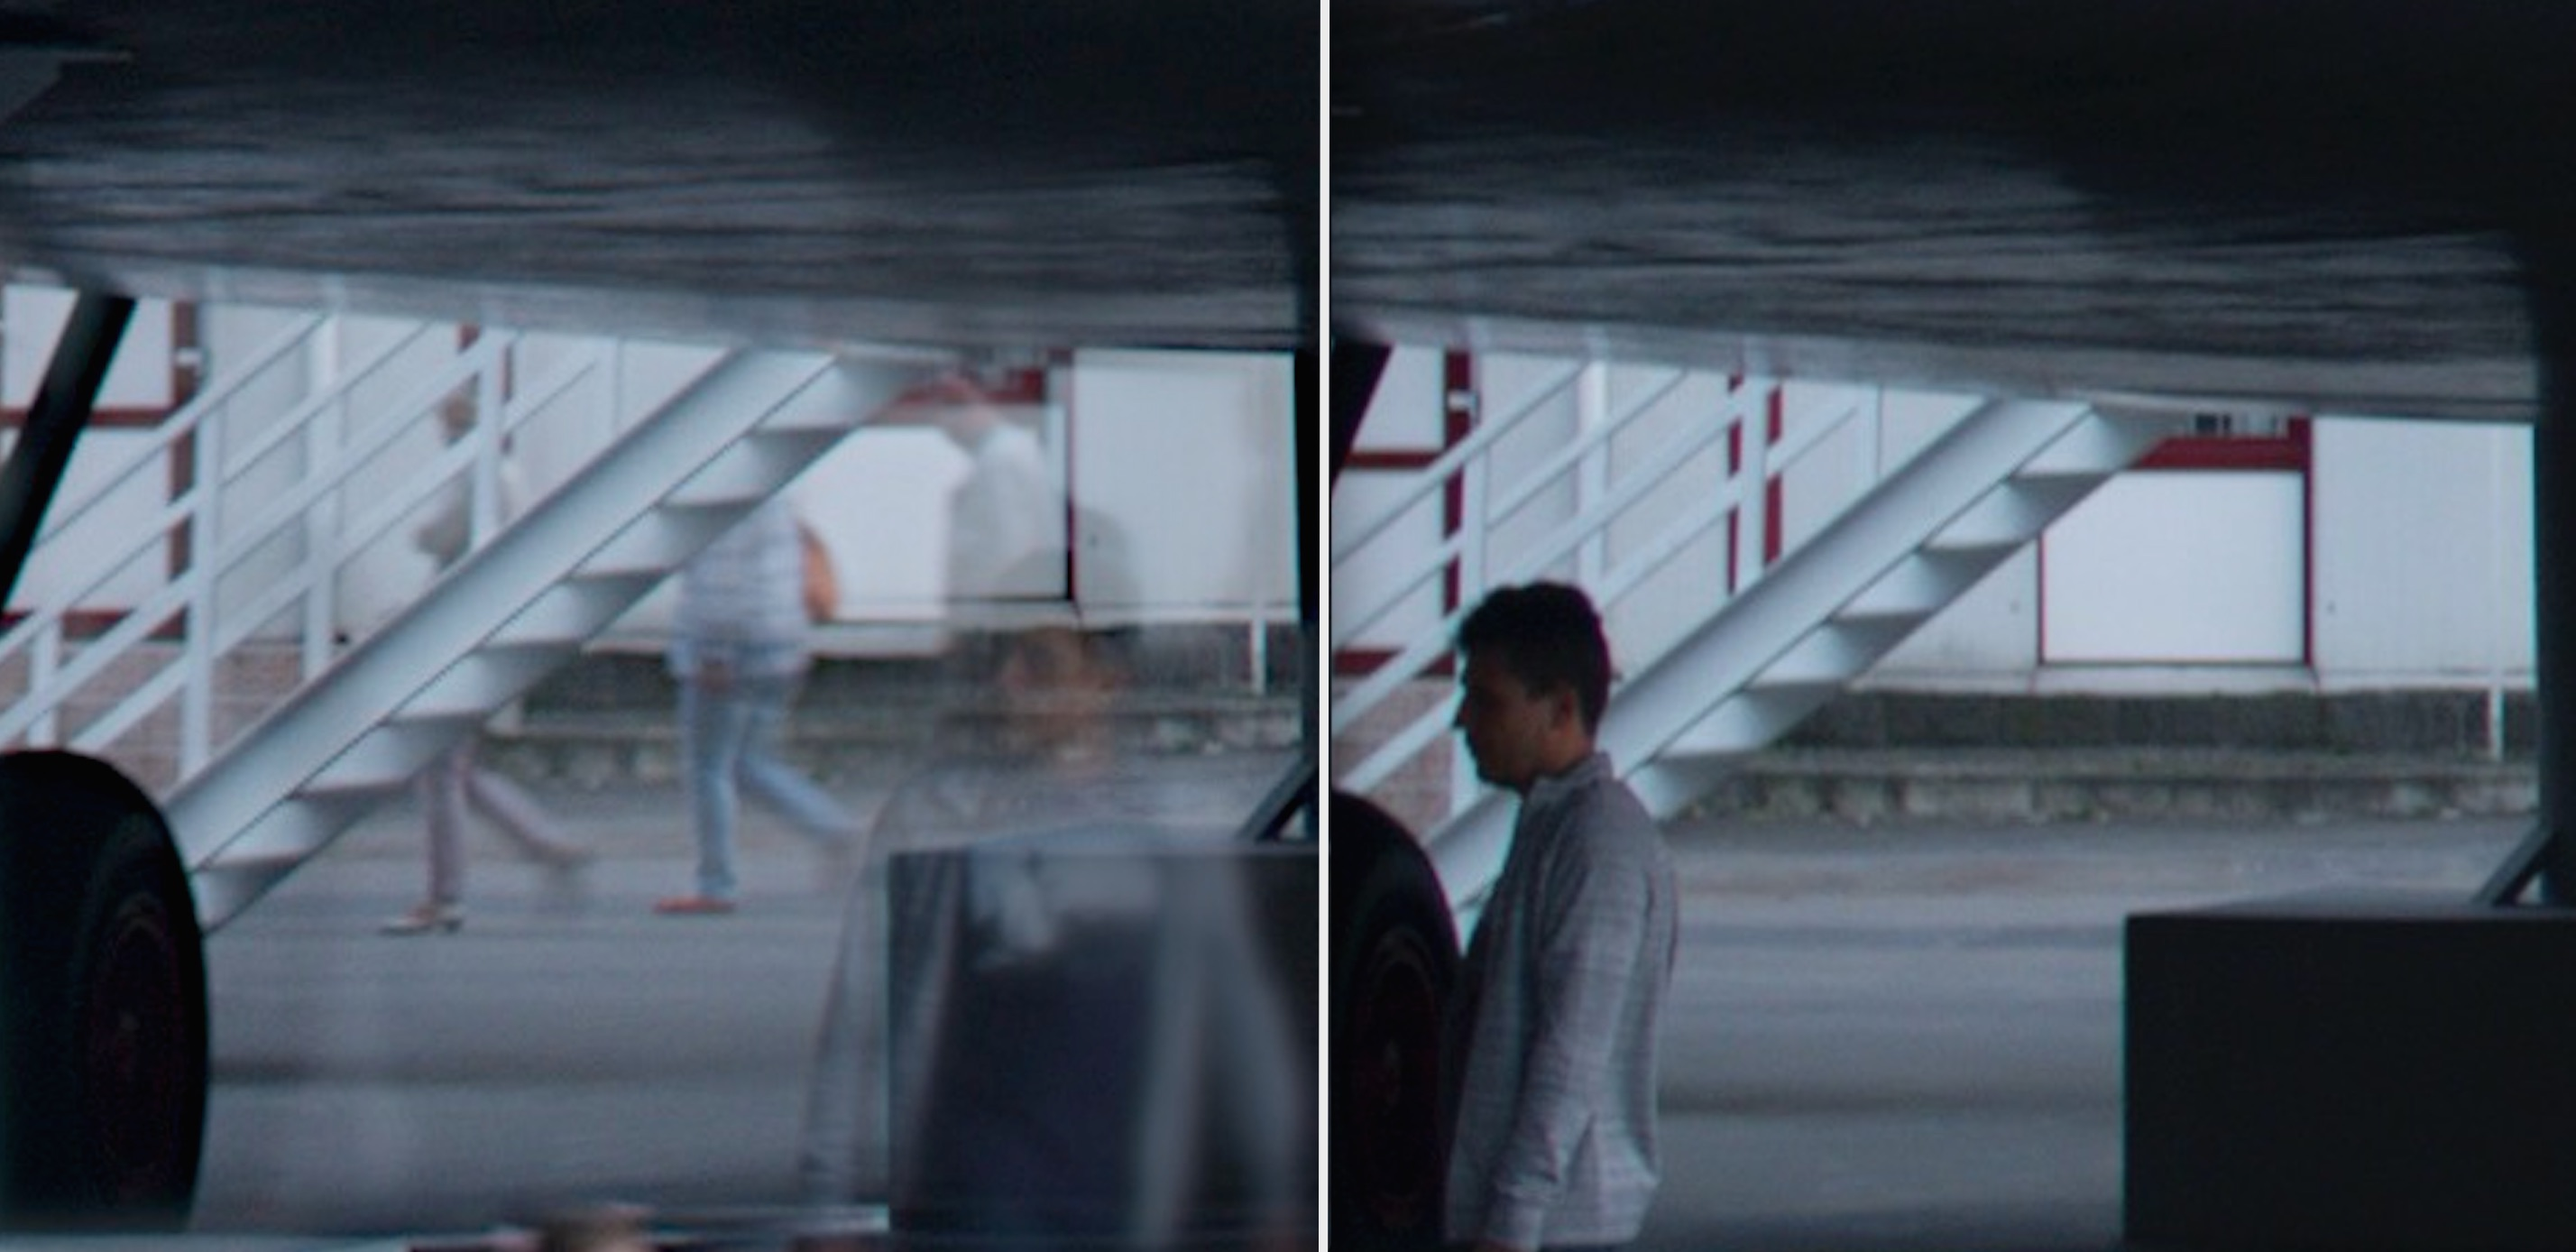
\includegraphics[width=1\textwidth]{img/ghosting.jpg}
	\caption{ Изображение с удаленными артефактами движущегося объекта(справа), артефакты на необработанном изображении(слева)}
        \label{fig:ghosting}
        }
\end{figure}

Во время съемки видео такие артефакты могут значительно повлиять на отображаемую информацию исходной каратинки. Чтобы этого не допустить требуется позаботиться об удалении избыточной информации перед слиянием кадров с разной экспозицией.

В статье \cite{bib5} рассматриваются разные решения удаления артефактов при получении HDR изображения. По результатам их исследований алгоритм BMD является наиболее оптимальным в получении изображения с динамически расширенным диапазоном.

\subsection { Алгоритм BMD(Bitmap Movement Detection)}

Алгоритм BMD\cite{bib5} основывается на использовании MTB\cite{bib4} растрового изображения. Использование побитовых операций позволяет добиться быстрой скорости и точности вычислений.В качестве результата алгоритм предоставляет \textit{ Размеченную матрицу движений}. С помощью этой матрицы при склеивании кадров с разной экспозицией можно будет удалить артефакты.

Первым делом требуется найти для каждого изображения MTB растровое изображения. Пусть $B_i$ -- массив этих растровых изображений. На неподвижной, статичной сцене предполагается, что каждый пиксель сохраняет свое значение на всех растровых изображениях, хранящихся в $B_i$. Очевидно, что если значение пикселя поменяется, в области пикселя произошло движение. 

Суммируя все растровые изображения из $B_i$ между собой, получается $M^*$, в которой любые значения кроме 0 или N(количество исходных изображений) рассматриваются как совершенное движение в районе пикселя. 

$M^*$ может содержать некоторое количество шумов, которые могут повлечь за собой неприятные последствия -- некорректное определение области движения. Использование размытия по Гауссу позволяет значительно уменьшить шумы. Таким образом $M^*$ переводится в $M$ -- матрицу движений \ref{fig:bmdExample}.

\begin{figure}[!tbp]
  \centering
  \begin{subfigure}{.5\textwidth}
    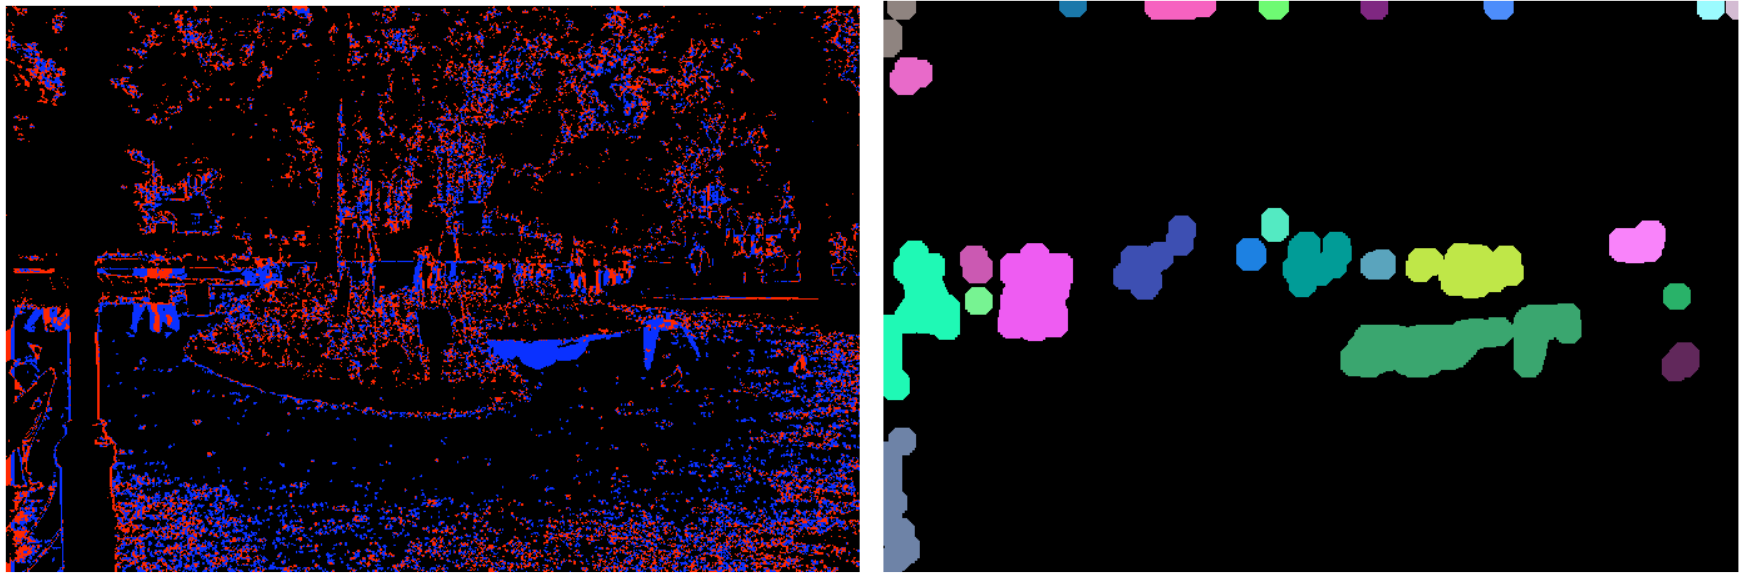
\includegraphics[width=\textwidth]{img/motionMap.png}
    \caption{ Представление матрицы движений(справа), и матрицы движений до преобразований(из-за большого количества шума сложно понять где и что передвигается).}
  \end{subfigure}\hfill
  \begin{subfigure}{.3\textwidth}
    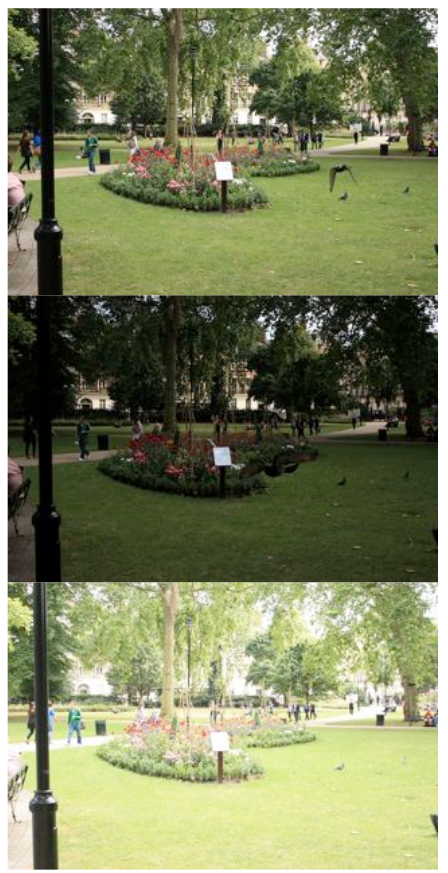
\includegraphics[width=\textwidth]{img/exposureSet.png}
    \caption{ Исходная последовательно изображений с разными экспозициями.}
  \end{subfigure}
  \caption { Пример нахождения движений на последовательности изображений с разными экспозициями.}
  \label{fig:bmdExample}
\end{figure}

Затем матрица движений переводится в кластерное отображение, которое получается с помощью Connected Component labeling, где у каждого кластера есть своя метка. Отсюда получается размеченная карта движений $L_M$ с размеченными кластерными зонами $\Omega_i$, которые содержат пиксели, влияющие на появлиение артефактов.

\section{ Получение HDR изображения}

Целью данной работы является получение HDR изображение на LDR мониторах, которые не в состоянии отобразить широкий диапазон яркостей. В связи с этим наиболее подходящим алгоритмом в получении такой картинки является \textit{слияние экспозиций}\cite{bib7}. Данный метод позволяет получить сразу LDR изображение с динамически расширенным диапазоном без применения tonemmapping.

\subsection { Слияние экспозиций}

С помощью слияния экспозиций изображение выстраивается из "лучших" частей входных изображений с разными экспозициями. Оно рассчитывается с помощью матрицы весов. Исходные изображения объединяются, опираясь на нее(изображение \ref{fig:weights}. Каждое значение матрицы весов основывается на трех главных параметрах: контрасте, насыщенности и на экспозиционном значении.

\begin{figure}[!tbp]
  \centering
  \begin{subfigure}{.5\textwidth}
    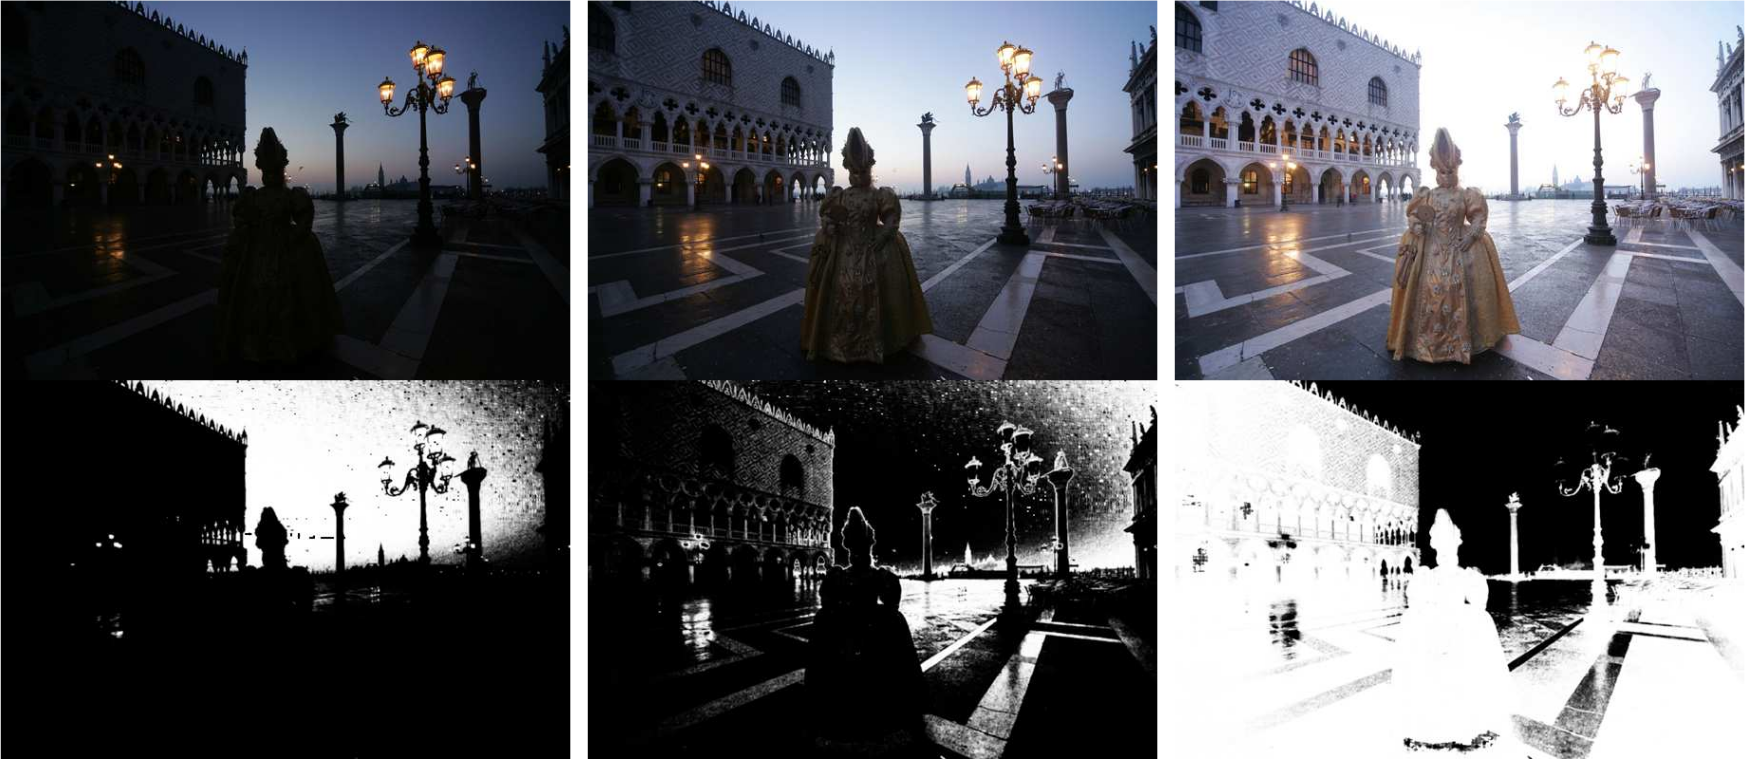
\includegraphics[width=\textwidth]{img/weights.png}
    \caption{ Входные изображения с соответствующими матрицами весов}
    \label{fig:weights}
  \end{subfigure}\hfill
  \begin{subfigure}{.5\textwidth}
    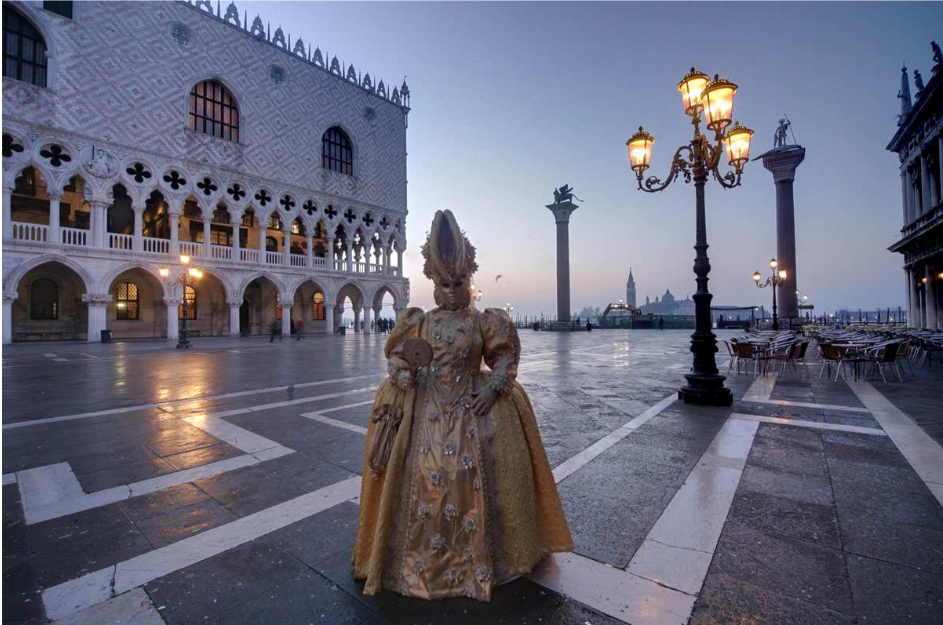
\includegraphics[width=\textwidth]{img/weightsResult.png}
    \caption{ Изображение после слияния кадров}
  \end{subfigure}
  \caption { Пример построение изображения путем слияния кадров.}
  \label{fig:weightsResult}
\end{figure}

\begin{enumerate}
   \item \textbf{Контраст:} каждое входное изображение переводится в монохромное и на него накладывается фильтр Лапласса. Абсолютное значение каждого элемента полученной матрицы будет являтся контрастностью \textit{C} соответствующего пикселя.
    \item \textbf{Насыщенность:} Насыщенностью \textit{S} будет являтся различие красного, зеленого и синого каналов каждого пикселя.
    \item \textbf{Значение экспозиции:} Значения интенсивностей каналов показывает на сколько хорошо выстроенна экспозиция пикселя. Интенсивности должны лежать между нулем(засвеченное изображение) и еденицей(слишком темное изображение). Каждая интенсивность канала рассчитывается с помощью уравнения \ref{eq:well-exposedness}, в котором определяется на сколько близко значение лежит к 0.5 с помощью кривой Гаусса.
\end{enumerate}

\begin{equation}
    \centering{
        E = \exp{\Big(-\frac{(i-0.5)^2}{2*\sigma^2}\Big)}}
    \label{eq:well-exposedness}
\end{equation}

, где \textit{i} - интенсивность канала, \textit{$\sigma$} - константа, равняющаяся 0.2.

Вычисления выше используются для построения матрицы весов и вычисляются для каждого пикселя путем перемножения всех трех параметров: контрастности, насыщенности и значения экспозиции. Таким образом, в одном значении матрицы весов учитываются все эти параметры. Вычисление значений матрицы весов представлено в \ref{eq:weightedValue}

\begin{equation}
    \centering{
        W_{ij,k} = (C_{ij,k})^{\omega_{C}} \times (S_{ij,k})^{\omega_{S}} \times (E_{ij,k})^{\omega_{E}}}
    \label{eq:weightedValue}
\end{equation}

,где C, S и E - контраст, насыщенность и значение экспозиции соответственно. \textit{$\omega_{C}$}, \textit{$\omega_{S}$} и \textit{$\omega_{E}$} - параметры, с помощью которых регулируется приоритет того или иного значения. \textit{ij, k} - (i, j) пиксель \textit{k}-того изображения. Если значение $\omega$ равняется 0, то соответствующее значение не учитывается. Полученный вес пикселя \textit{$W_{ij,k}$} будет использоваться при слиянии кадров.

Для слияния N изображений вначале высчитывается среднее значение веса каждого пикселя. Вычисление среднего значения веса представлено в выражении \ref{eq:averageWeight}

\begin{equation}
    \centering{
        \overset{^\wedge}{W_{ij,k}} = \Big[\sum_{k'=1}^{N}W_{ij,k'}\Big]^{-1}W_{ij,k}}
    \label{eq:averageWeight}
\end{equation}

Для дальнейшего слияния изображений используется алгоритм пиромидальной декомпозиции изображения(пирамида Гаусса и пирамида Лапласса)\cite{bib8}, который позволяет получить отфильтрованные изображения в разных разрешениях. Затем производится слияние кадров на каждом из уровней пирамиды. 

Получить результирующее изображение с произведенным слиянием можно с помощью выражения \ref{eq:pyrExposureFusion}

\begin{equation}
    \centering{
        L\{R\}_{ij}^{l} = \sum_{k=1}^{N}G\{\overset{^\wedge}{W}\}_{ij,k}^{l}L\{I\}_{ij,k}^{l}}
    \label{eq:pyrExposureFusion}
\end{equation}

Где \textit{l} - уровень пирамиды декомозированного изображения, а \textit{$L\{A\}^l$} - декомпозиция изображения \textit{A} на \textit{l} уровне пирамиды Лапласса и $G{B}^l$ - декмопозиция изображения \textit{B} на уровне \textit{l} пирамиды Гаусса. Пример такой декомпозиции представлен на изображении \ref{fig:expfusion}

\begin{figure}[ht!]
    \centering{
        \includegraphics[width=1\textwidth]{img/exposureFusion.png}
	\caption{ Представление процесса слияния экспозиций}
        \label{fig:expfusion}
        }
\end{figure}

Самый нижний уровень пирамиды $L\{R\}$ и будет являться результатом слияния экспозиций - $R$.
